\subsection{Misceláneos}

\subsubsection{Conectar Tierras}

Es importante conectar las tierras (GND) de nuestros dispositivos. Hasta este punto, sólo falta conectar un pin GND del arduino con un pin negativo del Model Y board. 

\subsubsection{Bocina}

Colocar la bocina en algún espacio sobre el acrílico superior. Conectar un pin de la bocina con el pin 8 del arduino. El otro pin creo que es conectarlo a tierra del arduino.

\subsubsection{Cámara}

Tener el módulo de cámara para la raspberry pi (es decir, tener la cámara), el cuál se ilustra en la figura \ref{fig:cam}. Luego insertarla en el puerto del módulo de cámara, este puerto se ilustra en la figura \ref{fig:pcam}. Imágenes tomadas de \href{https://projects.raspberrypi.org/en/projects/getting-started-with-picamera/1URL}{https://projects.raspberrypi.org/en/projects/getting-started-with-picamera/1}.

\begin{figure}[htbp]
    \centering
    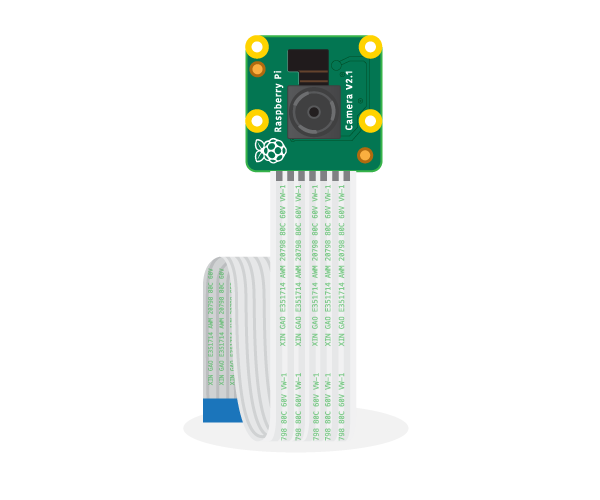
\includegraphics[width=0.3\textwidth]{imagenes/camera-module.png}
    \caption{Módulo de cámara para la raspberry pi.}
    \label{fig:cam}
\end{figure}

\begin{figure}[htbp]
    \centering
    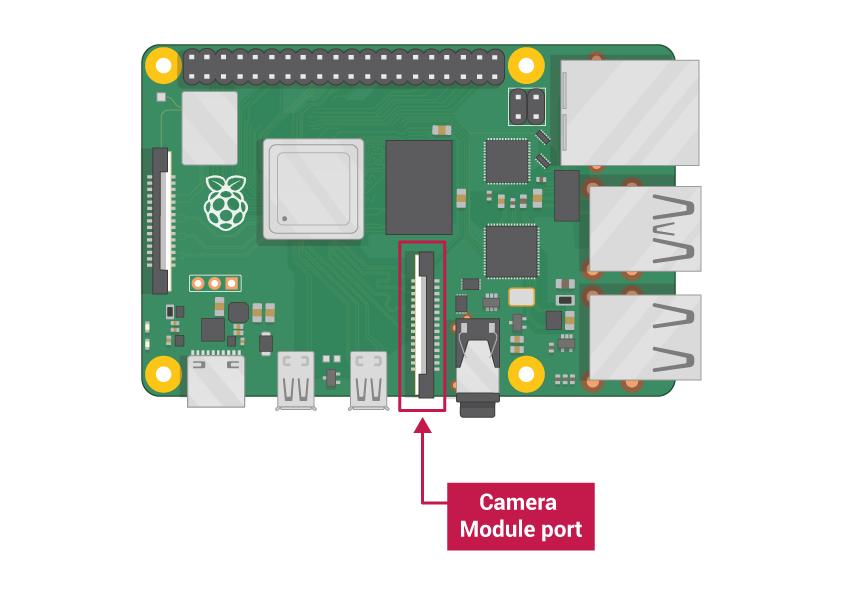
\includegraphics[width=0.3\textwidth]{imagenes/pi4-camera-port.png}
    \caption{Puerto para el módulo de cámara}
    \label{fig:pcam}
\end{figure}
